\begin{enumerate}[label=\thechapter.\arabic*,ref=\thechapter.\theenumi]
\item The frequency response $H(f)$ of of a linear time-invariant syatem has magnitude as shown in \figref{fig:11}\\
Statement 1: The system is necessarily a pure delay system for inputs which are bandlimited to $-a \leq f \leq a$.\\
Statement 2: For any wide-sense stationary input process with power spectral density $S_X(f)$, the output power spectral density $S_Y(f)$ obeys $S_X(f)=S_Y(f)$ for $-a \leq f \leq a$.\\
\begin{figure}[!ht]
\centering
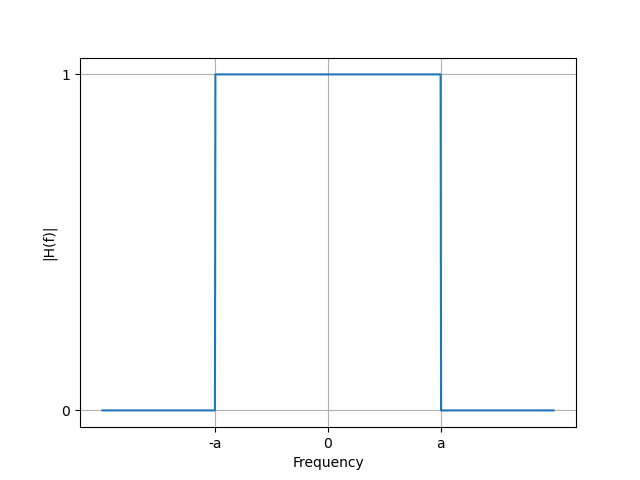
\includegraphics[width=\columnwidth]{gate/EC/2022/23/figs/figure.png}
\caption{$|H(f)|$ vs frequency}
\label{fig:23.2022,1}
\end{figure}\\
\iffalse
\let\negmedspace\undefined
\let\negthickspace\undefined
\documentclass[journal,12pt,twocolumn]{IEEEtran}
\usepackage{cite}
\usepackage{amsmath,amssymb,amsfonts,amsthm}
\usepackage{algorithmic}
\usepackage{graphicx}
\usepackage{textcomp}
\usepackage{xcolor}
\usepackage{txfonts}
\usepackage{listings}
\usepackage{enumitem}
\usepackage{mathtools}
\usepackage{gensymb}
\usepackage{comment}
\usepackage[breaklinks=true]{hyperref}
\usepackage{tkz-euclide} 
\usepackage{listings}
\usepackage{gvv}                                        
\def\inputGnumericTable{}                                 
\usepackage[latin1]{inputenc}                                
\usepackage{color}                                            
\usepackage{array}                                            
\usepackage{longtable}                                       
\usepackage{calc}                                             
\usepackage{multirow}                                         
\usepackage{hhline}                                           
\usepackage{ifthen}                                           
\usepackage{lscape}

\newtheorem{theorem}{Theorem}[section]
\newtheorem{problem}{Problem}
\newtheorem{proposition}{Proposition}[section]
\newtheorem{lemma}{Lemma}[section]
\newtheorem{corollary}[theorem]{Corollary}
\newtheorem{example}{Example}[section]
\newtheorem{definition}[problem]{Definition}
\newcommand{\BEQA}{\begin{eqnarray}}
\newcommand{\EEQA}{\end{eqnarray}}
\newcommand{\define}{\stackrel{\triangle}{=}}
\theoremstyle{remark}
\newtheorem{rem}{Remark}
\begin{document}

\bibliographystyle{IEEEtran}
\vspace{3cm}

\title{Probability Assignment}
\author{EE22BTECH11022-G.SAI HARSHITH$^{*}$% <-this % stops a space
}
\maketitle
\newpage
\bigskip
\renewcommand{\thefigure}{\theenumi}
\renewcommand{\thetable}{\theenumi}

Question: The frequency response $H(f)$ of of a linear time-invariant syatem has magnitude as shown in \figref{fig:11}\\
Statement 1: The system is necessarily a pure delay system for inputs which are bandlimited to $-a \leq f \leq a$.\\
Statement 2: For any wide-sense stationary input process with power spectral density $S_X(f)$, the output power spectral density $S_Y(f)$ obeys $S_X(f)=S_Y(f)$ for $-a \leq f \leq a$.\\
\begin{figure}[!ht]
\centering
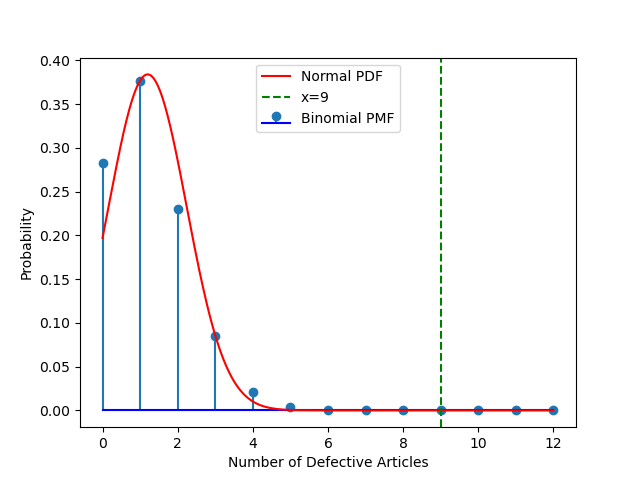
\includegraphics[width=\columnwidth]{figs/figure.png}
\caption{$|H(f)|$ vs frequency}
\label{fig:11}
\end{figure}\\
\fi
\solution A system where output signal is a delayed version of input signal with no other transformations or operations is called a pure delay system.
\begin{enumerate}
\item Let us consider a LTI system with x(t) and y(t) as input and output signal. Let $T_d$ be delay between input and output. So,
\begin{align}
y(t)&=x(t-T_d)
\end{align}
Here $Y(f)$ and $X(f)$ are output and input signals in frequency domian. Let $H(f)$ be 
\begin{align}
H(f)&=\frac{Y(f)}{X(f)}\\
&=e^{-2\pi fjT_d}\\
\label{eq:23.2022,2}
|H(f)|&=1\\
\angle H(f)&=-2\pi fT_d
\end{align}
The system will acts as pure delay system for frequency $f$. Now, if we take $f^2$ as frequency, the system doesn't act as pure delay system.\\
Example : Consider 
\begin{align}
H(f)=e^{-2\pi f^2jT_d}
\end{align}
Appling inverse fourier transform to get time responce.
\begin{align}
h(t)&=\int_{-\infty}^{\infty}H(f)e^{2\pi jft}df\\
&=\sqrt{\frac{T_d}{it}}e^{-\brak{\frac{i\pi t}{T_d}}} \ne \delta(t-T_d)
\end{align}
Therfore system doesn't necessarily be pure delay.
So, Statement 1 is incorrect.
\item For wide-sense stationary LTI sytem, Spectral power density of a signal describes the power present in the signal as a function of frequency, per unit frequency. In frequency domain,
\begin{align}
S_X(f)&=|X(f)|^2
\label{eq:23.2022,9}\\
S_Y(f)&=|Y(f)|^2
\label{eq:23.2022,10}
\end{align}
Dividing \eqref{eq:23.2022,9} and \eqref{eq:23.2022,10}.
\begin{align}
S_Y(f)&=\left|\frac{Y(f)}{X(f)}\right|^2S_X(f)\\
&=|H(f)|^2S_X(f)
\end{align}
From \eqref{eq:23.2022,2}, for $-a \leq f \leq a$,
\begin{align}
S_Y(f)&=(1)^2S_X(f)\\
S_Y(f)&=S_X(f)
\end{align}
Statement 2 is correct.
\end{enumerate}

\hfill (GATE EC 2022)
\end{enumerate}
